\documentclass[11pt]{ctexart}
\usepackage[margin=2.4cm]{geometry}
\usepackage{graphicx}
\usepackage{siunitx}
\usepackage{booktabs}
\usepackage{amsmath}
\usepackage{xcolor}
\usepackage{caption}
\usepackage[colorlinks=true,linkcolor=blue!60!black,urlcolor=blue!60!black]{hyperref}
\sisetup{detect-all, per-mode=symbol}

\definecolor{good}{HTML}{2E7D46}
\definecolor{bad}{HTML}{B23B3B}

\title{\bfseries 32\,导 ADS1299 脑电帽:\\阻抗模式与 \SI{31.2}{\hertz} 电流注入的实证验证}
\author{EEG\_MI 项目}
\date{2026 年 7 月 22 日}

\begin{document}
\maketitle

\begin{abstract}
\noindent
厂商未在文档中说明阻抗模式,我们此前仅从逆向反编译的采集软件\emph{推断}出:发送 \texttt{'\%'} 命令会让板子注入一个 \SI{31.2}{\hertz} 的交流电流。本报告用一个 \textbf{A/B/A 三段协议}在真机上做了实测,结论:\textbf{(1)} 阻抗模式确实存在——一个强而窄的 \SI{31.2}{\hertz} 谱峰\emph{仅}出现在阻抗模式,回到 EEG 模式立即消失;\textbf{(2)} 反推出注入电流为\textbf{纳安级($\sim$\SI{24}{\nano\ampere}),而非此前误称的微安级};\textbf{(3)} 解释了一个反直觉现象——\emph{不戴帽子时幅度只有约 \SI{1}{\milli\volt},戴上后反而升到约 \SI{10}{\milli\volt}}——其根本原因是\textbf{注入回路是否闭合},这同时也解释了厂商的绝对阻抗公式为何不可信。
\end{abstract}

\section{背景与问题}
本项目使用一顶 32 通道干电极脑电帽(TI ADS1299,WiFi/UDP)。厂商固件里有一个未公开的\textbf{阻抗模式}:采集软件向板子发送 \texttt{'\%'} 后,界面会显示每个电极的"接触强度"。我们通过逆向其 PyInstaller 打包的采集程序,读到它的做法是:测量每通道在 \SI{31.2}{\hertz} 处的电压幅度 $V_1$,再用一个线性公式换算成阻抗。

问题是:\emph{这只是从代码里读出的推断,我们从未真正测量过这个 \SI{31.2}{\hertz} 注入是否真实存在}。此外,实际使用中还观察到一个反直觉现象:\textbf{电极悬空(没戴)时 \SI{31.2}{\hertz} 幅度约 \SI{1000}{\micro\volt},戴到头上后反而升到约 \SI{10000}{\micro\volt}}。本报告用实测数据回答这两个问题。

\section{方法:A/B/A 三段协议}
脚本 \texttt{src/acquisition/test\_injection.py} 依次采集三段数据,每段数秒:
\begin{center}
\begin{tabular}{@{}cll@{}}
\toprule
段 & 模式(命令) & 预期 \\
\midrule
A & EEG 模式(\texttt{'*'}) & \textbf{无} \SI{31.2}{\hertz} 谱线 \\
B & 阻抗模式(\texttt{'\%'}) & 每通道出现\textbf{强而窄}的 \SI{31.2}{\hertz} 谱线 \\
C & EEG 模式(\texttt{'*'},恢复) & \SI{31.2}{\hertz} 谱线\textbf{消失} \\
\bottomrule
\end{tabular}
\end{center}

\noindent\textbf{内置对照:}\SI{50}{\hertz} 工频在三段中都存在。它证明了频谱是真实采到的、通道在正常工作,从而把"某个巧合的 \SI{31}{\hertz} 噪声"这一可能性排除掉——\emph{只有 \SI{31.2}{\hertz} 分量是随模式开关的}。对每段计算全通道平均幅度谱、每通道在注入频率的幅度、以及信噪比。脚本每次运行后都会\textbf{强制恢复 EEG 模式}。

\section{结果:阻抗模式确实存在}
图~\ref{fig:inj} 是真机测得的四联图。

\begin{figure}[h]
\centering
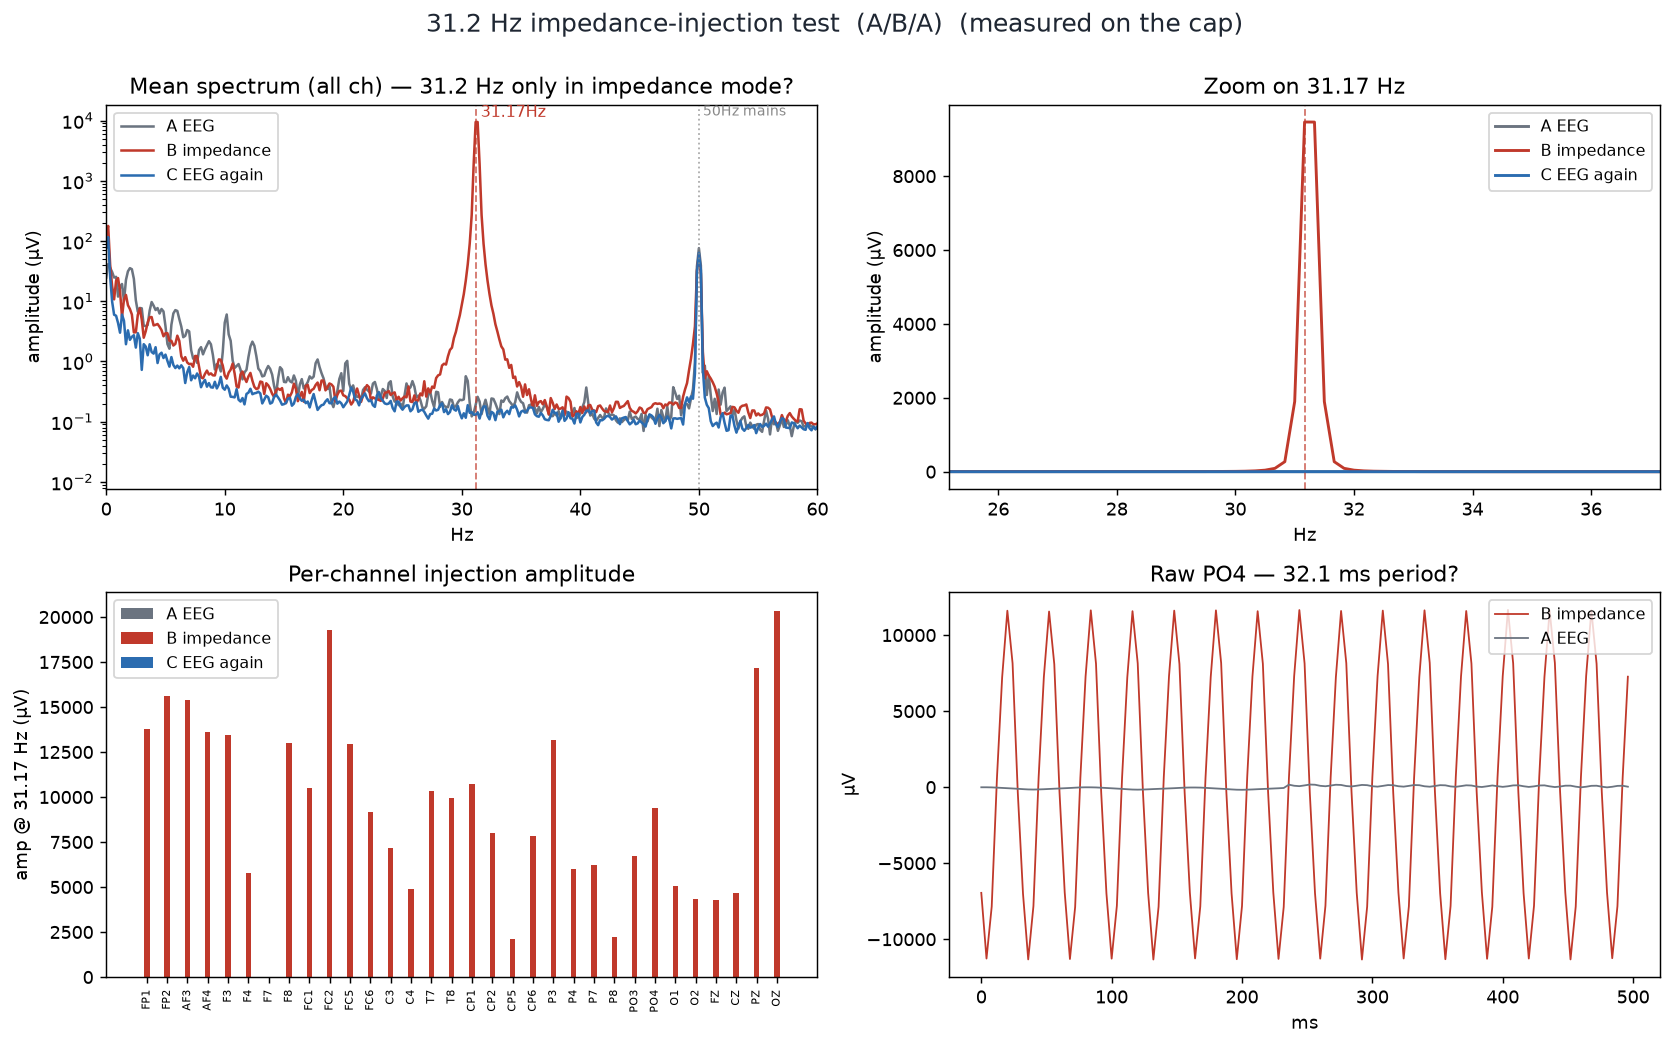
\includegraphics[width=\linewidth]{injection_test.png}
\caption{真机 A/B/A 实测。\textbf{左上:}全通道平均幅度谱(对数纵轴)——阻抗模式(红,B)在 \SI{31.17}{\hertz} 有一个高达 $\sim$\SI{e4}{\micro\volt} 的巨峰,两段 EEG 模式(灰 A、蓝 C)在该处什么都没有;\SI{50}{\hertz} 工频三段皆有(对照)。\textbf{右上:}放大后可见 $\sim$\SI{9500}{\micro\volt} 的尖峰仅在 B 段。\textbf{左下:}每通道注入幅度——所有通道在 B 段都被注入(\SIrange{2}{20}{\milli\volt}),EEG 段近于零。\textbf{右下:}PO4 原始波形——阻抗模式下是清晰的\textbf{三角波}($\pm\SI{11}{\milli\volt}$,周期 $\sim$\SI{32}{\milli\second}),EEG 模式下平直。}
\label{fig:inj}
\end{figure}

\noindent 三点观察确立结论:
\begin{enumerate}
\item \SI{31.17}{\hertz}($\approx f_s/8 = \SI{31.25}{\hertz}$,即由采样率数字分频而来)的谱峰\textbf{只在阻抗模式 B 出现},A 与 C 均无;
\item 该峰\textbf{遍布所有 32 个通道};
\item \SI{50}{\hertz} 工频三段一致,作为对照证明测量本身可信。
\end{enumerate}
\noindent\textbf{因此:阻抗模式真实存在,且由 \texttt{'\%'} / \texttt{'*'} 命令控制。}此前基于逆向的推断得到了实测证实。

\section{反推注入电流:是纳安级,不是微安级}
注入法阻抗就是欧姆定律 $Z=V/I$,其中 $I$ 由 ADS1299 的恒流源设定。有\textbf{两条独立证据}把电流量级钉在\textbf{纳安}级。

\paragraph{证据一:幅度量级。}戴帽后单通道幅度约 \SI{10}{\milli\volt}(PO4 峰值 $\pm\SI{11}{\milli\volt}$,OZ $\sim$\SI{20}{\milli\volt}),且\textbf{远未到 $\pm\SI{187.5}{\milli\volt}$ 的满量程}(没有削顶饱和),说明恒流源工作在线性区。用 $Z=V/I$ 反推,要产生 \SI{10}{\milli\volt} 所需的电极阻抗为:

\begin{center}
\begin{tabular}{@{}lcc@{}}
\toprule
假设注入电流 $I$ & 所需电极阻抗 $Z=V/I$ & 对干电极是否合理 \\
\midrule
\SI{24}{\micro\ampere} & $\approx \SI{420}{\ohm}$ & \textcolor{bad}{\textbf{否}}——干电极不可能这么低 \\
\SI{24}{\nano\ampere} & $\approx \SI{420}{\kilo\ohm}$ & \textcolor{good}{\textbf{是}}——干电极很典型 \\
\SI{6}{\nano\ampere} & $\approx \SI{1.7}{\mega\ohm}$ & \textcolor{good}{是}——干电极偏高但可能 \\
\bottomrule
\end{tabular}
\end{center}

\noindent 若真是 \SI{24}{\micro\ampere},则 \SI{10}{\milli\volt} 对应 \SI{420}{\ohm}——对任何头皮干电极都荒谬;反之若是 \SI{24}{\nano\ampere},对应 \SI{420}{\kilo\ohm},完全符合干电极量级。\textbf{故注入电流是几到几十纳安(基本就是 ADS1299 的 \SI{24}{\nano\ampere} lead-off 档),绝非 \SI{24}{\micro\ampere}。}

\paragraph{证据二:三角波形。}图~\ref{fig:inj} 右下的 PO4 波形是标准\textbf{三角波},而非正弦。三角波是\textbf{恒流(方波电流)对电容充放电}的特征:$I = C\,\mathrm{d}V/\mathrm{d}t$,恒定电流使电压\emph{线性}爬升,得到三角波。这直接说明:(i) 它是\textbf{电流源};(ii) 干电极在 \SI{31.2}{\hertz} 上是\textbf{电容主导}的。由斜率
\[
\frac{\mathrm{d}V}{\mathrm{d}t}\approx\frac{\SI{22}{\milli\volt}}{\SI{16}{\milli\second}}\approx \SI{1.4}{\volt\per\second},\qquad
I = C\cdot\frac{\mathrm{d}V}{\mathrm{d}t},
\]
取干电极双电层电容 $C\sim\SIrange{10}{20}{\nano\farad}$,得 $I\sim\SIrange{14}{28}{\nano\ampere}$,与证据一一致。

\paragraph{如何精确定值。}要得到\emph{确切}的电流,唯一干净的办法是\textbf{已知电阻标定}:把一个已知电阻(如 \SI{100}{\kilo\ohm})接到输入端测 $V_1$,纯电阻给出方波响应,$I=V_1/R$ 直接得出,且避开了电极电容的干扰。

\section{为什么"没戴 $\sim$1000,戴上反而 $\sim$10000"}
这正是最反直觉、也最能说明问题的一点。\textbf{教科书式的串联阻抗测量} $V=I\cdot Z$ 中,阻抗越高电压越高;那么\emph{电极悬空(阻抗趋于无穷)本应读到最高电压},而实测恰恰\textbf{相反}。这说明本板测的\textbf{不是干净的单电极串联阻抗,而是注入回路能否导通、耦合是否良好}。

\begin{quote}
恒流源在某电极注入 \SI{31.2}{\hertz} 电流,该电流必须经\\
\centerline{\textbf{电极 $\to$ 头皮 $\to$ 身体 $\to$ 参考/BIAS 电极 $\to$ 回到板子}}\\
形成\textbf{闭合回路},才能在电极上建立起可测的电压。
\end{quote}

\begin{itemize}
\item \textbf{没戴(悬空):}回路是\textbf{断开}的(没有身体通路),几乎没有电流真正流过。此时测到的 $\sim$\SI{1000}{\micro\volt} 只是电极/走线之间的\textbf{杂散电容耦合},并非真实的注入电压。
\item \textbf{戴上:}电极与参考电极都接触头皮,回路\textbf{闭合},恒流真正流过,$V=I\cdot Z$ 出现,幅度跳到 $\sim$\SI{10}{\milli\volt}。
\item \textbf{按压:}接触更好、回路耦合更强 $\Rightarrow$ 幅度更高。
\end{itemize}

\noindent 换言之,本板上 \SI{31.2}{\hertz} 幅度衡量的是\textbf{注入耦合 / 接触好坏},\textbf{越高 $=$ 接触越好}——这与串联阻抗方向\emph{相反}(悬空阻抗无穷本应最高,实测却最低),正说明主导因素是\textbf{回路是否导通},而非单电极的串联 $Z$。

\paragraph{对厂商阻抗公式的直接启示。}厂商用形如 $Z=a\,V+b$ 的线性式反推绝对阻抗,\emph{隐含假设"电压随接触阻抗单调上升"}(接触越差电压越高)。但真机行为是\textbf{反的、且非单调的}(接触越差/悬空,电压越低)。用一个连方向都搞反的公式去反推绝对 \si{\kilo\ohm},自然会得到负值,两个版本的公式也会互相矛盾(实测其斜率对应的注入电流相差约 $600\times$,见图~\ref{fig:formula})。\textbf{结论:绝对 \si{\kilo\ohm} 不可信;用 \SI{31.2}{\hertz} 相对幅度判断接触才是对的。}

\begin{figure}[h]
\centering
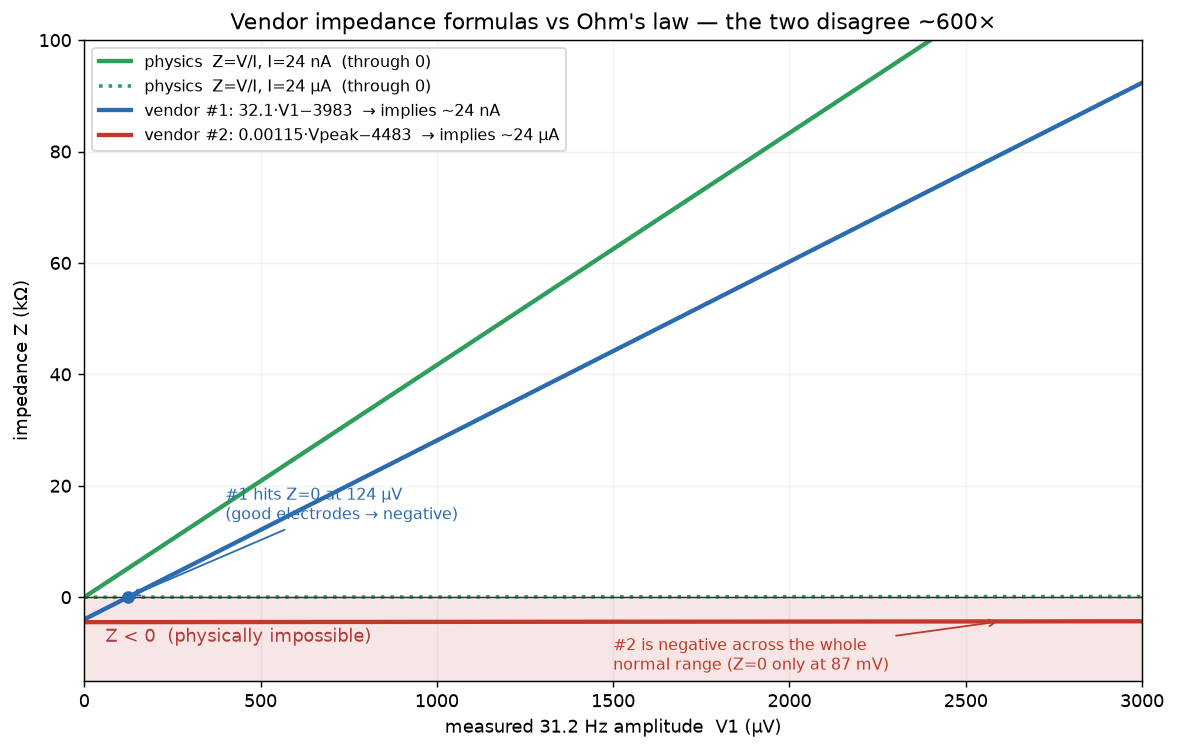
\includegraphics[width=0.82\linewidth]{impedance_formula_analysis.png}
\caption{厂商两个阻抗公式与欧姆定律 $Z=V/I$(过原点)的对比。两个公式都带\textbf{负截距}(好电极会算出负阻抗,粉色不可能区),且其斜率反推出的注入电流相差约 $600\times$(公式\#1 $\Rightarrow\sim$\SI{24}{\nano\ampere},公式\#2 $\Rightarrow\sim$\SI{24}{\micro\ampere}),\textbf{二者不可能同时成立}。}
\label{fig:formula}
\end{figure}

\section{结论}
\begin{enumerate}
\item \textbf{阻抗模式真实存在。}\SI{31.17}{\hertz}($\approx f_s/8$)注入谱峰仅在阻抗模式出现、遍布所有通道、并随 \texttt{'\%'}/\texttt{'*'} 开关;\SI{50}{\hertz} 对照确保测量可信。
\item \textbf{注入电流是纳安级($\sim$\SI{24}{\nano\ampere}),不是微安级。}由毫伏级幅度(未饱和)与三角波形两条独立证据得出;此前文档中的"\SI{24}{\micro\ampere}"应更正为"$\sim$\SI{24}{\nano\ampere}"。
\item \textbf{"没戴低、戴上高"源于注入回路的闭合。}悬空时回路断开、几乎无电流,只剩杂散耦合($\sim$\SI{1}{\milli\volt});戴上后回路闭合、恒流流过($\sim$\SI{10}{\milli\volt})。因此读数反映接触耦合(越高越好),与教科书串联阻抗方向相反——这也正是厂商绝对阻抗公式失效的根源。
\end{enumerate}

\vspace{1em}
\noindent\rule{\linewidth}{0.4pt}\\[2pt]
{\small \textbf{复现:}\; \texttt{python src/acquisition/test\_injection.py -{}-seconds 6}\;(连上 ESPBCI、确认 IP\,=\,192.168.4.2、关闭厂商 \texttt{main\_ui} 后运行)。图由 \texttt{src/acquisition/impedance\_formula\_check.py} 生成。}

\end{document}
